
% In low-resource academic setting, collecting a sufficient amount of data to potentially train an debug LLM will be cost prohibitive (est. cost XXX, with human labeling efforts). 
% Instead, we developed an effective LLM workflow via prompt design that is cost efficient.
% Note that our main purpose here is not to develop a SOTA debug LLM, instead, we aim to show that even with low-resource setting, our proposed TAXONOMY is highly effective in building a prompt based debug LLM workflow.


\begin{figure}[htbp]
    \centering
    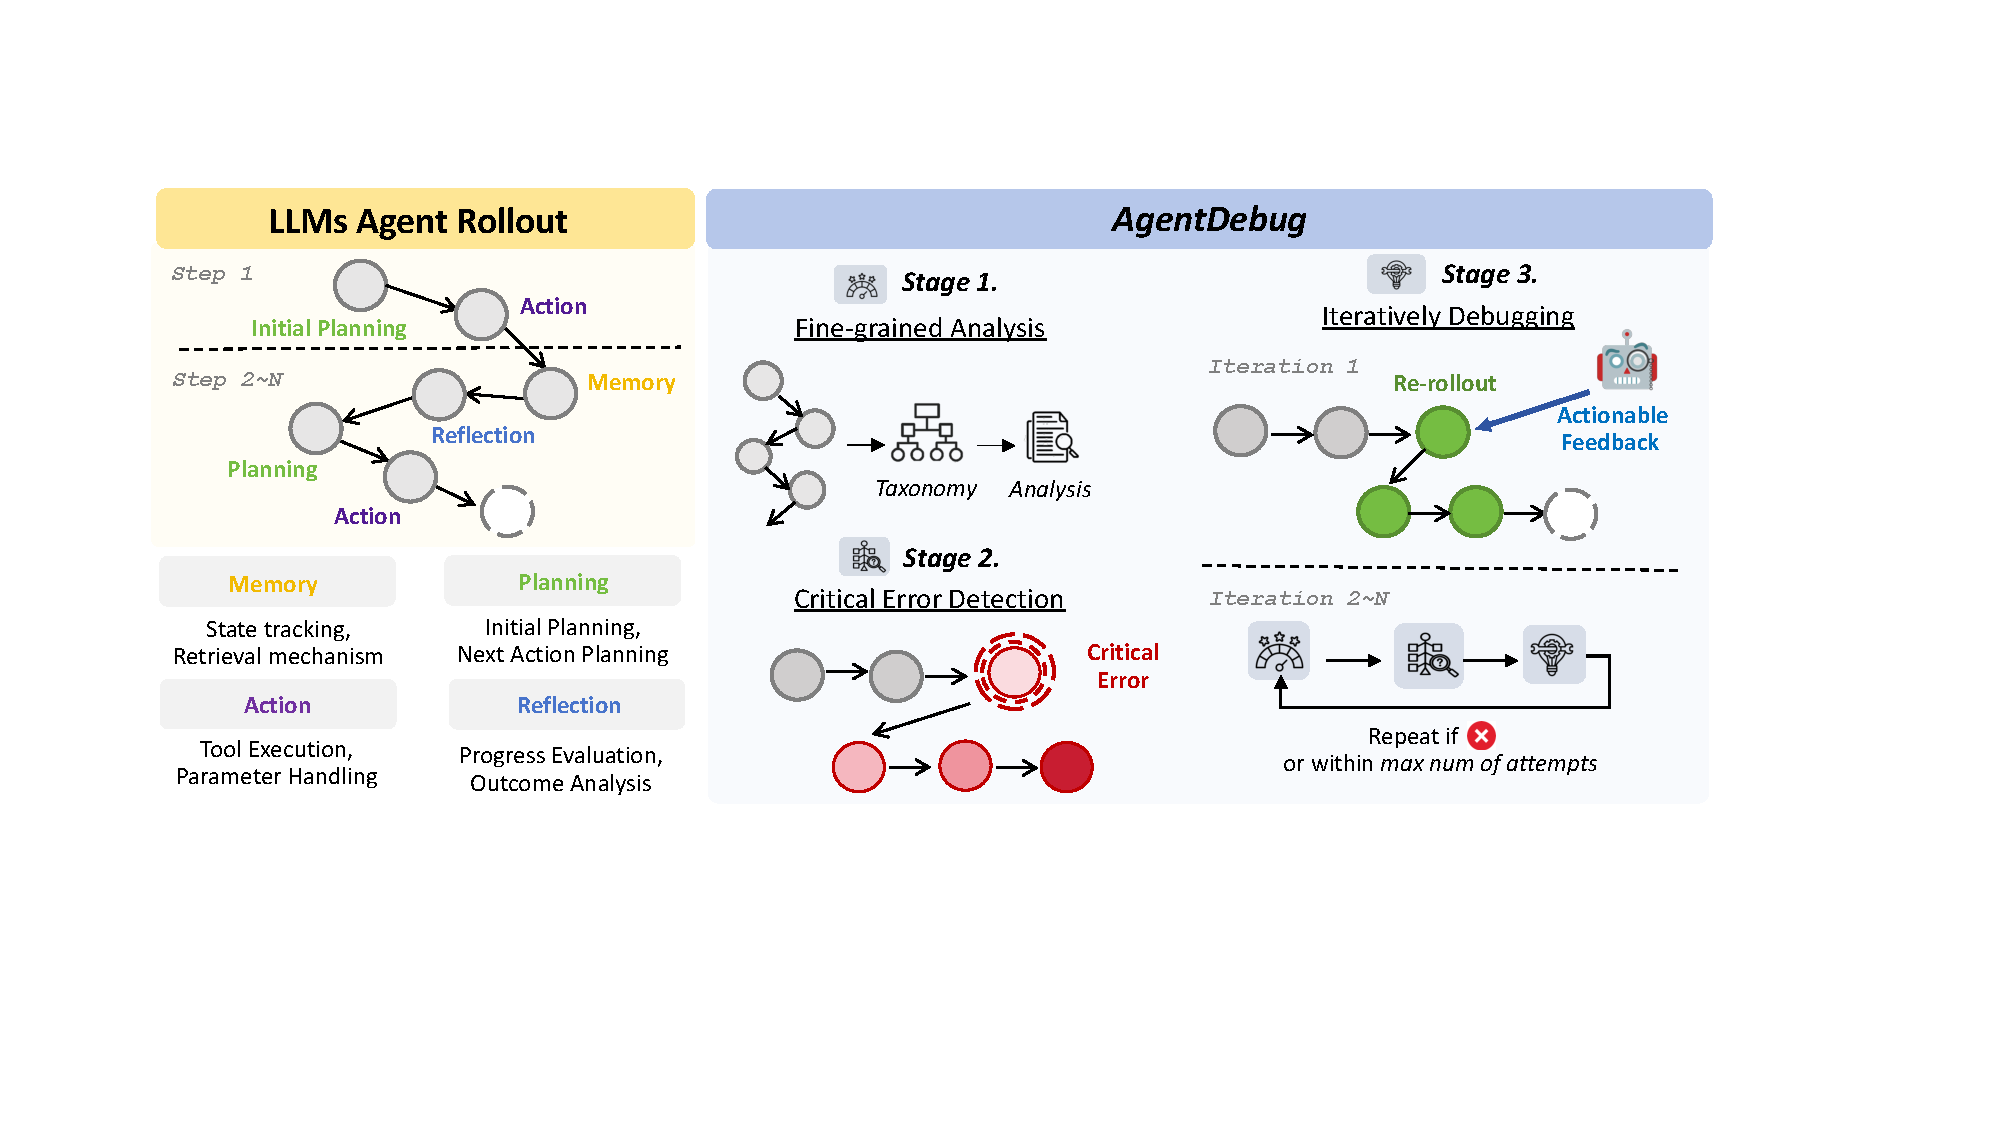
\includegraphics[width=1\linewidth]{figures/method.pdf}
    \caption{\textbf{Overview of \ModelName{}.} (Left) LLM agent rollouts alternate between memory, planning, reflection, and action. (Right) \ModelName{} debugs trajectories in three stages: (1) fine-grained analysis across steps and modules, (2) detection of the critical error that triggers failure, and (3) iterative re-rollouts with actionable feedback to turn failures into successes.}
    \label{fig:method}
\end{figure}


% \begin{algorithm}[h]
% \small
% \DontPrintSemicolon
% \SetAlgoLined
% \LinesNotNumbered
% \KwIn{Trajectory $\tau = \{(s_t, a_t)\}_{t=1}^T$; Error taxonomy $\mathcal{E}_{\text{AET}}$; Max Iterations $I$}
% \KwOut{Corrected trajectory $\tau^*$ \textbf{or} \texttt{Failure}}

% \SetKwFunction{Eval}{Eval}
% \SetKwFunction{MapAET}{MapToAET}
% \SetKwFunction{Correct}{CorrectAction}
% \SetKwFunction{Replace}{ReplaceAction}
% \SetKwFunction{Reroll}{ReRollout}
% \SetKwFunction{GenFB}{GenFeedback}
% \SetKwFunction{UpdFB}{UpdateFeedback}

% \tcc{Stage 1: Fine-grained Analysis with AET}
% \For{$t \gets 1$ \KwTo $T$}{
%   \ForEach{$m \in \{\text{mem}, \text{plan}, \text{refl}, \text{act}\}$}{
%     $e_t^m \gets \MapAET(s_t,a_t,m,\mathcal{E}_{\text{AET}})$ \tcp*{Assign error type per module}
%   }
% }
% \If{\Eval{$\tau$} $=1$}{\Return $\tau$ \tcp*{Trajectory already successful}}

% \tcc{Stage 2: Critical Error Detection via Counterfactuals}
% $t^* \gets \varnothing$ \;
% \For{$t \gets 1$ \KwTo $T$}{
%   $\hat{a}_t \gets \Correct(s_t,a_t,\{e_t^m\}_{m})$ \tcp*{Generate corrected action}
%   $\hat{\tau} \gets \Replace(\tau,t,\hat{a}_t)$ \;
%   \If{\Eval{$\hat{\tau}$} $=1$}{
%     $t^* \gets t$ \tcp*{Earliest correction that removes final failure}
%     \textbf{break}
%   }
% }
% \If{$t^*=\varnothing$}{\Return \texttt{Failure} \tcp*{No critical error found}}

% \tcc{Stage 3: Iterative Debugging with Targeted Feedback}
% $\phi^{(0)} \gets \GenFB(s_{t^*},a_{t^*},\{e_{t^*}^m\}_{m})$ \tcp*{Actionable feedback}
% $\tau^{(0)} \gets \tau$ \;
% \For{$k \gets 1$ \KwTo $I$}{
%   $\tau^{(k)} \gets \Reroll(\tau^{(k-1)}, t^*, \phi^{(k-1)})$ \tcp*{Re-execute from $t^*$ with feedback}
%   \If{\Eval{$\tau^{(k)}$} $=1$}{\Return $\tau^{(k)}$}
%   $\phi^{(k)} \gets \UpdFB(\tau^{(k)}, \phi^{(k-1)})$ \tcp*{Refine guidance if still failing}
% }
% \Return \texttt{Failure} \tcp*{Max Attempts Reached}
% \caption{\ModelName{} Inference Procedure}
% \label{alg:model}
% \end{algorithm}

\begin{algorithm}[h]
\small
\DontPrintSemicolon
\SetAlgoLined
\LinesNotNumbered
\KwIn{Trajectory $\tau = \{(s_t, a_t)\}_{t=1}^T$; Error taxonomy $\mathcal{E}_{\text{AET}}$; Critical-error criterion $\mathcal{C}_{\text{crit}}$; Max Iterations $I$}
\KwOut{Corrected trajectory $\tau^*$ \textbf{or} \texttt{Failure}}

\SetKwFunction{Eval}{Eval}
\SetKwFunction{MapAET}{MapToAET}
\SetKwFunction{Reroll}{ReRollout}
\SetKwFunction{GenFB}{GenFeedback}
\SetKwFunction{UpdFB}{UpdateFeedback}
\SetKwFunction{Detect}{DetectCriticalErrors}

\tcc{Stage 1: Fine-grained Analysis with AET}
\For{$t \gets 1$ \KwTo $T$}{
  \ForEach{$m \in \{\text{mem}, \text{plan}, \text{refl}, \text{act}\}$}{
    $e_t^m \gets \MapAET(s_t,a_t,m,\mathcal{E}_{\text{AET}})$ \tcp*{Assign error type per module}
  }
}
\If{\Eval{$\tau$} $=1$}{\Return $\tau$ \tcp*{Trajectory already successful}}

\tcc{Stage 2: Critical Error Detection via LLM (no rollout/counterfactuals)}
$\mathcal{C} \gets \{\tau,\{e_t^m\}_{t,m},\mathcal{E}_{\text{AET}},\mathcal{C}_{\text{crit}}\}$ \tcp*{Pack analysis, taxonomy \& criterion}
$(\mathcal{T}^*, \mathcal{M}^*, \mathcal{Z}^*, \phi^{(0)}) \gets \Detect(\mathcal{C})$ \tcp*{LLM (fine-grained prompt)}
\If{$\mathcal{T}^*=\varnothing$}{\Return \texttt{Failure} \tcp*{No critical error found}}
$t^* \gets \min(\mathcal{T}^*)$ \tcp*{Earliest critical step}
\tcp{$\mathcal{T}^*$: set of critical steps; $\mathcal{M}^*$: modules per critical step; $\mathcal{Z}^*$: error-types per critical step}

\tcc{Stage 3: Iterative Debugging with Targeted Feedback}
$\tau^{(0)} \gets \tau$ \;
\For{$k \gets 1$ \KwTo $I$}{
  $\tau^{(k)} \gets \Reroll(\tau^{(k-1)}, t^*, \phi^{(k-1)})$ \tcp*{Re-execute from $t^*$ with feedback}
  \If{\Eval{$\tau^{(k)}$} $=1$}{\Return $\tau^{(k)}$}
  $\phi^{(k)} \gets \UpdFB(\tau^{(k)}, \phi^{(k-1)})$ \tcp*{Refine guidance if still failing}
}
\Return \texttt{Failure} \tcp*{Max Iterations Reached}
\caption{\ModelName{} Inference Procedure }
\label{alg:model}
\end{algorithm}


Building on our analysis of agent failures, we aim to develop method that actively refine themselves by learning from mistakes. We first formalize the key modules of an LLM-based agent in Section~\ref{sec:rollout}, and then present our proposed framework, \ModelName{}, in Section~\ref{sec:model}.


\subsection{Key Modules of an LLM Agent}
\label{sec:rollout}
As illustrated in Figure~\ref{fig:method}, we consider an agent that interacts with an environment over a sequence of steps.  
At each step, the agent observes a state and produces an action, forming a trajectory of state–action pairs.  
Each action is generated through four sequential modules: \textbf{Memory}, which recalls relevant past information; \textbf{Reflection}, which evaluates progress and interprets feedback; \textbf{Planning}, which formulates the next strategy; and \textbf{Action}, which executes the low-level operation.  
Errors can occur in any of these modules, and mistakes made early often propagate through later stages, compounding into larger failures.  This modular rollout design not only mirrors the agent’s internal decision process, but also provides a natural structure for human annotators to align errors with specific modules, making the diagnosis of agent failures more transparent and interpretable.  

\subsection{\ModelName{} Framework}
\label{sec:model}
We propose \ModelName{}, a debugging framework that enables single-LLM agents to diagnose and recover from their own failures across diverse environments. As illustrated in Fig.~\ref{fig:method}, \ModelName{} analyzes complete trajectories to (i) assign fine-grained error types to each step and module, (ii) identify the earliest critical error that directly causes the final failure, and (iii) provide actionable feedback to guide re-rollouts. The central intuition is that correcting a single root-cause mistake can often flip an otherwise failing trajectory into a successful one.

As presented in Algorithm~\ref{alg:model}, the inference procedure of \ModelName{} consists of three stages:

\paragraph{Stage 1: Fine-grained Analysis with \AET{}.}  
For each step in the trajectory, we analyze all four modules—memory, reflection, planning, and action.  
Each module is mapped to an \AET{} error type, grounding the analysis in interpretable categories such as “constraint ignorance” or “format error.”  
This produces a structured, module-level error profile for the trajectory.  

\paragraph{Stage 2: Critical Error Detection via Counterfactuals.}  
If the trajectory is already successful, no debugging is required.  
Otherwise, we perform counterfactual testing step by step: at each point, we substitute a corrected action and test whether the rollout would succeed.  
The \emph{critical error} is defined as the earliest step whose correction directly prevents the final failure.  
Unlike superficial mistakes or errors that are later corrected, the critical error is the root cause that truly determines whether the overall trajectory succeeds or fails—capturing both \emph{when} and \emph{why} the agent goes irreversibly off track.  

\paragraph{Stage 3: Iterative Debugging with Targeted Feedback.}  
Once the critical error is identified, the system generates feedback that specifies the error type and provides actionable guidance for refining subsequent actions and plans.  
The agent then re-executes (re-rolls out) the trajectory under this feedback. If the rollout still fails, the feedback is refined with more specific guidance, and the process repeats up to a fixed budget of attempts.  
Grounded in the \AET{} taxonomy, the feedback is both targeted and forward-looking—resolving the root cause while shaping how the agent approaches future steps.  



